%\documentclass[aps,pra,amsmath,amssymb,floatfix,twocolumn, amsmath, superscriptaddress, twocolumn]{revtex4}
%\documentclass[aps,amsmath,prl]{revtex4-2}
\documentclass{report}
\usepackage{multirow}
\usepackage{bbold}
\usepackage{subfigure}
\usepackage{color}
\usepackage{mathrsfs}
\usepackage{a4wide}
%\usepackage{hyperref}

\newcommand{\pg}[1]{\textcolor{red}{#1}}
\newcommand{\bvec}[1]{{\mathbf #1}}
%\newcommand{\bra}[1]{\left< #1 \right|}
%\newcommand{\ket}[1]{\left| #1 \right>}


\usepackage{amsfonts, relsize, color}
\usepackage{graphics}
\usepackage{graphicx}
\usepackage{subfigure}
\usepackage{hyperref}
\usepackage{color}
\usepackage{physics}
\newcommand{\expect}[1]{#1}
\renewcommand\vec[1]{\ensuremath\boldsymbol{#1}} % bold font for vectors

%\usepackage[english]{babel}
\usepackage[utf8]{inputenc}
\usepackage{fancyhdr}
\usepackage[backend=bibtex]{biblatex}
%\usepackage{biblatex}
\addbibresource{references.bib}


\pagestyle{fancy}
\fancyhf{}

\rhead{Effects of Berry Curvature on Thermoelectric Transport ...}
\lhead{A. Panigrahi}
%\rfoot{Page \thepage}



\begin{document}


%\title{\bf Effects of Berry Curvature on Thermoelectric Transport of Bilayer Graphene and Other Materials}


%\author{Archisman Panigrahi}
%\affiliation{Indian Institute of Science, Bangalore 560012, India}
%
%\author{Subroto Mukerjee}
%\affiliation{Indian Institute of Science, Bangalore 560012, India}

%\date{\today}




%\maketitle
\title{
	\sc
	\Huge{Effects of Berry Curvature on Thermoelectric Transport}\\
	\Large{in}\\
	\Huge{Bilayer Graphene and Other Materials}
	\\[30pt]
	\large{A Thesis submitted for the completion of}
	\\[5pt]
	\large{requirements for the degree of}
	\\[10pt]
	\Large{Bachelor of Science (Research)}
	\\[10pt]
	\normalsize{by}
	\\[10pt]
	\large{Archisman Panigrahi}
	\\[5pt]
	\normalsize{Undergraduate Programme}
	\\[5pt]
	\normalsize{Indian Institute of Science}
	\\[5pt]
	\normalsize{SR No.}
	\normalsize{11-01-00-10-91-17-1-14503}
	\\[10pt]
	
\includegraphics[scale=0.12]{Logo.png}
	\\[10pt]
	\normalsize{Under the supervision of}
	\\[10pt]
	\large{Prof. Subroto Mukerjee}\\[5pt]
	\normalsize{Dept. Of Physics}\\[5pt]
	\normalsize{Indian Institute of Science}
	\date{June 2021}
}
\maketitle

%\begin{abstract}
%Todo\\
%1. Need to acknowledgment, etc.\\
%2. Write an introduction.\\
%3. Move the calculations related to Boltzmann Transport Equation to appendix.
%\end{abstract}

\tableofcontents

%\onecolumngrid


%%%%%%%%%%%%%%%%%%%%%%%%%%%%%%%%%%%%%%%%%%%%%%%%%%%%%%
%%%%%%%%%%%%%%%%%%%%%%%%%%%%%%%%%%%%%%%%%%%%%%%%%%%%%%
%%%%%%%%%%%%%%%%%%%%%%%%%%%%%%%%%%%%%%%%%%%%%%%%%%%%%%
%%%%%%%%%%%%%%%%%%%%%%%%%%%%%%%%%%%%%%%%%%%%%%%%%%%%%%
%%%%%%%%%%%%%%%%%%%%%%%%%%%%%%%%%%%%%%%%%%%%%%%%%%%%%%
%\newpage

\chapter{Introduction}
intro
\chapter{Berry curvature in reciprocal space}
Before we discuss Berry curvature, let us consider a concrete example, a spatially fixed spin-$\frac{1}{2}$ particle in a rotating magnetic field. Suppose the magnetic field is rotating in the $xy$ plane. This problem can be solved exactly. The time evolution of the system is governed by the Hamiltonian, $H = -\mu_{_B} \vec{B}\cdot\vec{\sigma}$, where the rotating magnetic field $\vec{B} = (\cos{\omega t}, \sin{\omega t},0)$, and $\vec{\sigma} = (\sigma_x, \sigma_y, \sigma_z)$ is a vector containing the Pauli matrices. With the initial condition that the spin is initially pointing parallel the magnetic field, along the $x$ axis, $\Psi(0) = \frac{1}{\sqrt{2}}\begin{pmatrix}
	1 \\
	1 
\end{pmatrix}$. When the magnetic field rotates very slowly compared to the timescale of evolution of the system, i.e., $\omega \ll \frac{\mu_{_B} B}{\hbar}$, it can be shown that the spin wavefunction evolves as, $\Psi(t) = \left[e^{-i\frac{\omega t}{2}} e^{i \frac{\mu_{_B} B}{\hbar}t}\right] \frac{1}{\sqrt{2}}\begin{pmatrix}
1 \\
e^{i\omega t} 
\end{pmatrix}$.

Then, after a complete revolution of the magnetic field, at time $T = \frac{2\pi}{\omega}$, the state evolves to,
$\Psi(T) = e^{-i \pi} e^{i \frac{\mu_{_B} B}{\hbar} T} \Psi(0)$.
Although the magnetic field returns to its initial value, the state acquires an additional phase factor of $e^{-i \pi} = -1$, in addition to the usual phase factor of $e^{i \frac{\mu_{_B} B}{\hbar} T}$ (because the system remains in the instantaneous eigenstate with energy eigenvalue $- \mu_{_B} B$).

This is an example of a geometric phase (also known as the \textit{Pancharatnam–Berry phase}), which is the additional phase acquired by an eigenstate, when a parameter of the Hamiltonian (here the magnetic field) is varied slowly compared to the timescale ($\sim \frac{\text{energy}}{\hbar}$) of the state.

It can be shown that (see chapter 10 of \cite{book:Griffiths2004IntroductiontoQM}) if the magnetic field subtends a solid angle $\Omega$ and returns to its initial value, the accumulated geometric phase for a spin-$s$ system would be $-s{\Omega}$. Here the magnetic field subtends a solid angle $2 \pi$ after rotating about the $xy$ plane, and it is a spin-$\frac{1}{2}$ system, and the geometric phase after the magnetic field completes a revolution is $-\pi$, just as we saw previously.


\subsection{Geometric Phase and Berry Curvature}
When the Hamiltonian of a system has a paramater $\vec{\lambda}$ which evolves slowly (compared to the timescale $\frac{\hbar}{\varepsilon}$ of a state $\ket{\varepsilon}$), an eigenstate of the Hamiltonian evolves as (\cite{BerryQuantalPhase1984}, also see chapter 10 of  \cite{book:Griffiths2004IntroductiontoQM} for derivation),

\begin{equation}~\label{Eq:BerryPhaseOriginal}
	\ket{\varepsilon(\vec{\lambda}(t))} = e^{i \gamma(t)} e^{-\frac{i}{\hbar} \int_0^t \varepsilon(\vec{\lambda}(t')) dt'} \ket{\varepsilon(\vec{\lambda}(0))}
\end{equation}
where the geometric phase $\gamma(t)$ is given by the expression $$\gamma(t) = i\int_{\vec{\lambda}_i}^{\vec{\lambda}_f} \bra{\varepsilon({\vec{\lambda}})}\nabla_{_{\vec{\lambda}}} \ket{\varepsilon({\vec{\lambda}})} \cdot d \vec{\lambda}.$$ Its value depends on the trajectory in the parameter space $\vec{\lambda}$, not just the endpoints. The real quantity $i\bra{\varepsilon({\vec{\lambda}})}\nabla_{_{\vec{\lambda}}}\ket{\varepsilon({\vec{\lambda}})} = \vec{A(\vec{\lambda})}$ is known as the Berry connection  \footnote{$\bra{\varepsilon({\vec{\lambda}})}\nabla_{_{\vec{\lambda}}} \ket{\varepsilon({\vec{\lambda}})}$ stands for $\int d\vec{r} \varepsilon_{_{\vec{\lambda}}}^* (\vec{r}) \nabla_{_{\vec{\lambda}}} \varepsilon_{_{\vec{\lambda}}}(\vec{r})$, where $\varepsilon_{_{\vec{\lambda}}}(\vec{r})$ is the suitably normalized position space wavefunction of $\ket{\varepsilon({\vec{\lambda}})}$.}, and its curl, $\vec{\Omega} = \nabla_{_{\vec{\lambda}}} \times \vec{A}$ is known as the Berry curvature.

While the overall phase of the state does not affect its physical observables, if we take a linear combination of such eigenstates, each of them would evolve with a different geometric phase, and the interference of such phase factors would indeed affect the physical properties of the system. We would now see how such a geometric phase manifests in electrons moving in a lattice, when an external electromagnetic field is applied.


\subsection{Geometric phase of electrons in a lattice}
Now, let us consider an electron in a periodic potential $V(\vec{r})$ (e.g. the potential due to a lattice, without any external electromagnetic fields). Its Hamiltonian is given by $\hat{H} = \frac{{\hat{\vec{p}}}^2}{2 m} + V(\hat{\vec{r}})$.

The eigenfunctions of this Hamiltonian are of the form,
$$\psi_{n, \vec{k}} (\vec{r}) = e^{i \vec{k}\cdot \vec{r}} u_{n,\vec{k}} (\vec{r})$$

Here $u_{n,\vec{k}} (\vec{r})$ is a function with the same periodicity as $V(\vec{r})$ (e.g. in a lattice, it would be periodic in every unit cell). The quantity $\hbar \vec{k}$ is known as the crystal momentum and $n$ is the band index. This result is known as Bloch's theorem (See chapter 8 of \cite{book:AshcroftMermin76}). The crystal momentum is a good quantum number for an electron in a lattice, and it is conserved upto a reciprocal lattice vector (times $\hbar$).
Now, we can rewrite the eigenvalue equation $\left[-\frac{\hbar^2}{2m}\nabla^2 + V(\vec{r}) \right] \psi_{n, \vec{k}}(\vec{r}) = \varepsilon_{n,\vec{k}} \psi_{n, \vec{k}}(\vec{r})$ as,
\begin{equation}~\label{Eq:effectiveBlochEquation}
	\left[\frac{\hbar^2}{2m}(\vec{k} - i \nabla)^2 + V(\vec{r}) \right]u_{n,\vec{k}} (\vec{r}) = \varepsilon_{n,\vec{k}} u_{n,\vec{k}} (\vec{r})
\end{equation}

In this equation, $\vec{k}$ is just a parameter in the effective Hamiltonian. When we apply an external electromagnetic field, the crystal momentum is not anymore a good quantum number. Its evolution is governed by the Lorenz force, (See Appendix \ref{app:crystal-momentum-time-evolution} for derivation)

\begin{equation} \label{Eq:evolution-of-k}
	\boxed{\hbar \dot{\vec{k}} = -e\left(\vec{E} + \langle\dot{\vec{r}}\rangle \times \vec{B} \right)}
\end{equation}

As $\vec{k}$ (now a parameter of the effective Hamiltonian in Eq. \ref{Eq:effectiveBlochEquation}) changes, it would give rise to a geometric phase, just like Eq. \ref{Eq:BerryPhaseOriginal}. After a small time interval $\Delta t$, $\vec{k}$ would evolve to $\vec{k} + \dot{\vec{k}} \Delta t$ (we write $\dot{\vec{k}} \Delta t = \Delta \vec{k} $), and the periodic part of the Bloch wavefunction labeled with $\vec{k}$ would evolve as 
\begin{equation}\label{Eq:u-n-k-time-evolution}
	u_{n, \vec{k}} \rightarrow e^{i \gamma(\Delta t)} e^{-i \frac{\varepsilon_{_{\vec{k}}} \Delta t}{\hbar}} u_{n, \vec{k}+\Delta \vec{k}},
\end{equation} where $\gamma(\Delta t) =\vec{A}(\vec{k}) \cdot \Delta \vec{k}$, and $ \vec{A}(\vec{k})=i \bra{u_{n,\vec{k}}}\nabla_{_{\vec{k}}} \ket{u_{n,\vec{k}}}$ is the Berry connection \footnote{ $\bra{u_{n,\vec{k}}}\nabla_{_{\vec{k}}} \ket{u_{n,\vec{k}}}$ stands for $\int_\text{unit cell} d\vec{r} u^*_{n,\vec{k}} (\vec{r}) \nabla_{_{\vec{k}}} u_{n,\vec{k}}(\vec{r})$, where the normalization of $u_{n,\vec{k}}(\vec{r})$ is chosen such that $\int_\text{unit cell} d\vec{r} |u_{n,\vec{k}} (\vec{r})|^2 = 1$.} in the reciprocal space. Again, for a state labeled with a single $\vec{k}$, this geometric phase is an overall global phase, which would not show up in physical observables. However, if we take a linear superposition of Bloch wavefunctions with different values of $\vec{k}$, each of them would evolve with a different geometric phase $\gamma_n (\vec{k}) = \int_{0}^{t} dt' \vec{A(\vec{k})} \cdot \frac{d \vec{k}}{dt'} $, and we would soon see that the interference of such phase factors would lead to many interesting effects.

After all, this geometric phase is an effect of the Hamiltonian non commuting with itself at different times, for different values of the parameter $\vec{k}$. It can be easily verified that the commutator of the Hamiltonian with itself, for two different values of $\vec{k}$, namely, $\vec{k}_1$ and $\vec{k}_2$,
$$
\left[\frac{\hbar^2}{2m}(\vec{k}_1 - i \nabla)^2 + V(\vec{r}), \frac{\hbar^2}{2m}(\vec{k}_2 - i \nabla)^2 + V(\vec{r}) \right] = -\frac{i \hbar^2}{m} (\vec{k}_1 - \vec{k}_2)\cdot\nabla V(\vec{r})
$$

\section{Effects of Berry Curvature}
\subsection{Modification of semiclassical equations of motion of a wavepacket}
The probability density of the wavefunction $\psi_{n, \vec{k}} (\vec{r}) = e^{i \vec{k}\cdot \vec{r}} u_{n,\vec{k}} (\vec{r})$ is not localized anywhere, it is periodic over all unit cells (the blue curve in Fig. \ref{fig:wavepacket-and-bloch-wave}). We can construct a wave packet by forming a linear superposition of many such states, such that the wavepacket is localized at some point $\vec{r}_0$ in the real space (the red curve in \ref{fig:wavepacket-and-bloch-wave}), and its crystal momentum is also localized around a value of $\hbar \vec{k}_0$.

Although this wavepacket is localized in both real space and (crystal) momentum space, it does not violate Heisenberg's uncertainty relation, because for this wave packet, the product of the uncertainties in position and (crystal) momentum, $\Delta \vec{r} \Delta \vec{k}$ is still greater than $\frac{1}{2}$. While the wavepacket is spread over many unit cells, its spatial variation $\Delta \vec{r}$ is much smaller than the dimensions of the system, and $\Delta \vec{k}$ is much smaller than the dimensions of the Brillouin zone. As a result, in laboratory scale, the wavepacket behaves like a classical particle, with an almost localized value of position and crystal momentum.

\begin{figure}[h!]
	\centering
	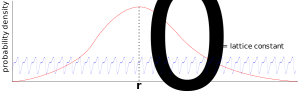
\includegraphics[width=0.7\linewidth]{wavepacket-and-Bloch-wave}
	\caption{The blue curve shows the probability density of a Bloch wavefunction. It is periodic over unit cells. The red curve shows a wavepacket which is localized in real space (although it is spread over many unit cells, it is localized compared to the dimensions of the system), as well as in crystal momentum space.}
	\label{fig:wavepacket-and-bloch-wave}
\end{figure}

It can be shown \cite{ralph2020berry} that for such a wavepacket, the expectation value of the position of its center evolves as,
\begin{equation}\label{Eq:evolution-of-r}
	\boxed{\langle\dot{\vec{r}}\rangle = \frac{1}{\hbar} \nabla{_{_{\vec{k}}}} \varepsilon_{_{\vec{k}}} - \langle\dot{\vec{k}}\rangle \times \vec{\Omega(\vec{k})}}
\end{equation}
Here, $\vec{\Omega(\vec{k})} = \nabla_{_{\vec{k}}} \times \vec{A(\vec{k})} = i \bra{\nabla_{_{\vec{k}}} u_{n,\vec{k}}}\times \ket{\nabla_{_{\vec{k}}} u_{n,\vec{k}}}$ is the Berry curvature in the reciprocal space. Also, here the energy eigenvalues are modified due to orbital magnetic moment $\vec{m}_{_{\vec{k}}}$ of an wavepacket (more about it in Section \ref{sec:OrbMagMom}) arising due to the Berry curvature, $\varepsilon_{_{\vec{k}}} = \varepsilon_0(\vec{k}) - \vec{m}_{_{\vec{k}}} \cdot \vec{B}$, where $\varepsilon_0(\vec{k})$ is the original bandstructure energy at zero magnetic field.

In popular Solid State Physics textbooks, the second term in the RHS of Eq. \eqref{Eq:evolution-of-r}, involving the Berry curvature is omitted (e.g. see Eq. 8.51 of \cite{book:AshcroftMermin76}). This is most likely because people thought that the overall phase factor is unimportant. Also, we would soon see that the Berry curvature is identically zero unless certain symmetries are broken, and this is why its effects cannot be experimentally observed in most systems. 

To see why the extra term appears, let us first investigate how we can produce such a wavepacket, which is localized in both position space and crystal momentum space. This discussion is based on Section I. of \cite{ralph2020berry}. To make the wavepacket localized near $\vec{k}_0$ in the reciprocal space, consider a \textit{real} weight function $w(\vec{k} - \vec{k}_0)$, which is sharply localized about $\vec{k} = \vec{k}_0$. Now consider a linear superposition of the Bloch wavefunctions, of the form, $\int d\vec{k} w(\vec{k} - \vec{k}_0) e^{-i \vec{k} \cdot \vec{r}_0 } \left(e^{i \vec{k} \cdot\vec{r}} u_{n,\vec{k}}\vec{r}\right)$. The expectation value of $\vec{k}$ of this wavefunction should be localized about $\vec{k}_0$. Then, near $\vec{r} = \vec{r}_0$, the functions $e^{i \vec{k} \cdot (\vec{r} -\vec{r}_0 )}$ constructively interfere, and we would expect the wavepacket to have a high probability density at $\vec{r}_0$. However, the functions $u_{n,\vec{k}}(\vec{r})$ may have different phases for different values of $\vec{k}$ at the same $\vec{r} = \vec{r}_0$, and then the waves would not constructively interfere.
After properly taking account of this (See Appendix \ref{app:calculation-of-<r>}), the wavefunction that is localized around $\expval{\vec{r}} = \vec{r}_0$, and peaked at crystal momentum $\hbar \vec{k}_0$ is found to be,
$$\psi(\vec{r}, t=0) = \int d\vec{k} w(\vec{k} - \vec{k}_0) e^{i \vec{A}(\vec{k_0})\cdot (\vec{k} - \vec{k}_0)} e^{-i \vec{k} \cdot \vec{r}_0 } \left(e^{i \vec{k} \cdot\vec{r}} u_{n,\vec{k}}(\vec{r})\right).$$
Here $\vec{A}$ is again the Berry connection. After a small time $\Delta t$, the individual Bloch wavefunctions would then evolve as in Eq. \eqref{Eq:u-n-k-time-evolution}, and the wavefunction of the wavepacket would be,
$$\psi(\vec{r}, t=\Delta t) = \int d\vec{k} w(\vec{k} - \vec{k}_0) e^{i \vec{A}(\vec{k_0})\cdot (\vec{k} - \vec{k}_0)} e^{-i \vec{k} \cdot \vec{r}_0 } \left(e^{i (\vec{k} + \Delta\vec{k})\cdot\vec{r}} e^{i \vec{A}\cdot \vec{\Delta{k}}} e^{-i \frac{\varepsilon_{_{\vec{k}}} \Delta t}{\hbar}} u_{n, \vec{k}+\Delta \vec{k}} \right).$$

It can be shown (See Appendix. \ref{app:center-at-new-time}), that for this state, the expectation value of position is located at
$$\langle \vec{r} \rangle = \vec{r}_0 +  \frac{\Delta t}{\hbar} \nabla{_{_{\vec{k}}}} \varepsilon_{_{\vec{k}}}|_{_{\vec{k} = \vec{k}_0}} - \Delta \vec{k}_0 \times \vec{\Omega(\vec{k}_0)}.$$
After dividing the shift in $\langle{\vec{r}}\rangle$ by $\Delta t$, Eq. \eqref{Eq:evolution-of-r} follows.
\subsection{Violation of Liouville's theorem and Modification of phase space density}
We now drop the notation $\expval{\cdot}$ of expectation values, and denote $\expval{\vec{r}} \equiv \vec{r}$ and $\expval{\vec{k}} \equiv \vec{k}$ for a wavepacket localized at $\vec{r}$ and $\vec{k}$. Consider a point $\left(\vec{r},\vec{k}\right)$ in the phase space, with a small volume element $\Delta V_0$ around it. The points inside the volume element $\Delta V_0$ evolve as governed by the semiclassical equations of motion,
\begin{equation}\label{Eq:evolution-of-R}
	\boxed{\dot{\vec{r}} = \frac{1}{\hbar} \nabla{_{_{\vec{k}}}} \varepsilon_{_{\vec{k}}} - \dot{\vec{k}} \times \vec{\Omega(\vec{k})}}
\end{equation}

\begin{equation}\label{Eq:evolution-of-K}
	\boxed{\hbar \dot{\vec{k}} = -e\left(\vec{E} + \dot{\vec{r}} \times \vec{B} \right)}
\end{equation}
and suppose, they occupy a new volume $\Delta V(t)$ around the point $\left(\vec{r'},\vec{k'}\right)$ after time $t$. Then, the quantity $$\Delta V(t) \left(1 + \frac{e}{\hbar} \vec{B}\left(\vec{r}(t)\right) \cdot  \vec{\Omega}\left(\vec{k}(t)\right)\right)$$ remains a constant of motion (See Appendix \ref{app:phase-space-volume-evolution}).

Liouville's theorem states that the volume $\Delta V$ occupied by a fixed number of points in the phase space remains invariant as the point $\left(\vec{r},\vec{k}\right)$ flows following the equations of motion (which are obtained from a classical Hamiltonian). In other words, the phase space density remains invariant. Here, that does not hold anymore (unless either of $\vec{B}$ or $\vec{\Omega}$ is zero, or they are orthogonal so that their dot product is zero). Note that the quantity defined above is a function of the local coordinates ($\vec{r}(t), \vec{k}(t)$), and does not depend on the trajectory.

Since the number of phase space points in the volume element $\Delta \vec{k} \Delta \vec{r} \left(1 + \frac{e}{\hbar} \vec{B}\left(\vec{r}(t)\right) \vec{\Omega}\left(\vec{k}(t)\right)\right)$ remains constant in time, if the magnetic field was initially zero, and we gradually turn on a homogeneous magnetic field, the number of states in the volume $\Delta \vec{k} \Delta \vec{r} \left(1 + \frac{e}{\hbar} \vec{B}(t) \cdot \vec{\Omega}\left(\vec{k}\right)\right)$ would be equal to the number of states in the initial volume $\Delta \vec{k} \Delta \vec{r}$.

As a result, when we calculate the expectation value of any operator $\mathcal{O}$ over all states, we would have to introduce an additional factor of $\left(1 + \frac{e}{\hbar} \vec{B} \cdot \vec{\Omega}\left(\vec{k}\right)\right)$ in the integrand, to correctly take account of all the states.
\begin{equation}~\label{Eq:operator-expval}
\expval{\mathcal{O}} = \int \frac{d\vec{k}}{(2\pi)^d} \left(1 + \frac{e}{\hbar} \vec{B} \cdot  \vec{\Omega}\left(\vec{k}\right)\right) \expval{\mathcal{O}}_{_{\vec{k}}} \tilde{g}_{\vec{k}}
\end{equation}

Here, $\tilde{g}_{\vec{k}}$, known as the distribution function, counts the occupation number of electrons in a state labeled with $\vec{k}$. When no external fields are applied, in thermodynamic equilibrium, it is the Fermi distribution function, $\tilde{g}_{_{\vec{k}}} = f_{_{\vec{k}}} = \frac{1}{e^{\beta \left(\varepsilon_{_{\vec{k}}} - \mu \right)} + 1}$. When an electromagnetic field is applied, this equilibrium is disturbed, and we write the distribution function as $\tilde{g}_{_{\vec{k}}} = f_{_{\vec{k}}} + g_{_{\vec{k}}}$, where $g_{_{\vec{k}}}$ is the non-equilibrium part of the distribution. We will see how to calculate it in Section \ref{sec:BTE-and-solution}.

Also, since Liouville's theorem does not hold anymore, we cannot obtain the equations of motion \eqref{Eq:evolution-of-R} and \eqref{Eq:evolution-of-K} from any effective Hamiltonian. 

\subsection{Orbital Magnetic moment}~\label{sec:OrbMagMom}
text
\section{When do we get a non-zero Berry Curvature?}
\subsection{Spatial Inversion Symmetry}
Under spatial inversion symmetry, the polar vectors change sign, $\vec{r} \rightarrow -\vec{r}$, $\vec{k} \rightarrow -\vec{k}$, $\vec{E} \rightarrow -\vec{E}$, but axial vectors like $\vec{B} \rightarrow \vec{B}$ remain unchanged. Also, since $\vec{\Omega} = \nabla_{_{\vec{k}}} \times A$ itself is an axial vector, under spatial inversion it changes as, $\vec{\Omega(\vec{k})} \rightarrow \vec{\Omega(\vec{-k})}$.

Then, if we apply the spatial inversion operator, the LHS of Eq. \eqref{Eq:evolution-of-r} changes sign, and then the RHS must change sign too. Then, $\dot{\vec{k}}\times \vec{\Omega(\vec{k})}$ must also change overall sign. But, under spatial inversion,  $\dot{\vec{k}}\times \vec{\Omega(\vec{k})} \rightarrow (-\vec{\dot{k}})\times \vec{\Omega(\vec{-k})}$, and this must be equal to $-\dot{\vec{k}}\times \vec{\Omega(\vec{k})}$, and we must have, 
\begin{equation}\label{Eq:OmegaSpatialInversion}
	\vec{\Omega}(-\vec{k}) = \vec{\Omega}(\vec{k}),
\end{equation}
when spatial inversion symmetry is present.\\\\

\subsection{Time Reversal Symmetry}
Under time reversal, the quantities $\vec{\dot{r}} \rightarrow -\vec{\dot{r}}$, $\vec{k} \rightarrow -\vec{k}$ change sign, whereas $\vec{\dot{k}} \rightarrow \vec{\dot{k}}$ remains the same. The spin of the electron also flips, $\vec{\sigma} \rightarrow -\vec{\sigma}$.

If we apply the time reversal operator, the LHS of Eq. \eqref{Eq:evolution-of-r} changes sign, and then $\dot{\vec{k}}\times \vec{\Omega(\vec{k})}$ must change an overall sign too. In general, the Berry curvature depends on the band index and the spin, and it follows that when time reversal symmetry is present,
\begin{equation}\label{Eq:OmegaTimeReversal}
	\vec{\Omega}_{n,\sigma}(-\vec{k}) = -\vec{\Omega}_{n,-\sigma}(\vec{k}).
\end{equation}

When there is no spin orbit coupling, the spatial parts of the wavefunctions for up and down spins are the same, consequently the Berry curvatures are the same too (because the Berry Curvature $\vec{\Omega}(\vec{k}) = i \bra{\nabla_{_{\vec{k}}} u_{n,\vec{k}}}\times \ket{\nabla_{_{\vec{k}}} u_{n,\vec{k}}}$ is a function of the spatial part of the wavefunction).

Then, when the spin orbit coupling is negligible, under time reversal symmetry,
\begin{equation}\label{Eq:OmegaTimeReversalzeroSpinOrbit}
	\vec{\Omega}_{n,\sigma}(-\vec{k}) = -\vec{\Omega}_{n,\sigma}(\vec{k}).
\end{equation}
\subsection{Conditions for non-Zero Berry Curvature}
As a result, when both spatial inversion and time reversal symmetry exist, and spin orbit coupling is negligible, then, combining Eq. \eqref{Eq:OmegaSpatialInversion} and Eq. \eqref{Eq:OmegaTimeReversalzeroSpinOrbit} $\vec{\Omega}_{n,\sigma}(-\vec{k}) = \vec{\Omega}_{n,\sigma}(\vec{k}) = -\vec{\Omega}_{n,\sigma}(\vec{k})$, i.e. $\vec{\Omega} \equiv 0$ for any $\vec{k}$.

Then, to get a non-zero Berry curvature \cite{ralph2020berry}, either time reversal or spatial inversion symmetry must be broken, or there must be significant spin orbit coupling. Note that these conditions are necessary to get a non-zero Berry curvature, but they may not be sufficient.

\subsection{Why the effects of Berry Curvature in transport took so long to be experimentally found?}
 In any metal, time reversal symmetry is already present, and the spatial inversion symmetry is present in BCC, FCC and simple cubic lattices. As a result, the Berry curvature is identically zero in most metals.
 
 Now we understand why the effects (e.g see section \ref{sec:AHE}) of the additional term in Eq. \eqref{Eq:evolution-of-R} were not seen in early transport experiments.
 
 A non-zero Berry curvature can present in biased Bilayer graphene, and also in topological materials like Chern Insulator and Weyl semimetal. These materials were experimentally realized in 21\textit{st} century.
 
 \textbf{CITE:} appropriate sources for Graphene and topological materials.
 
 \textbf{FIND:} more materials where there is a non-zero Berry curvature.

\section{Decoupling of the equations of motion and their simplification}

The differential equations of motion for $\dot{\vec{r}}$ and $\dot{\vec{k}}$ (Eq. \ref{Eq:evolution-of-R} and Eq. \ref{Eq:evolution-of-K}) can be easily decoupled (See Appendix \ref{app:decoupling-of-eom}), and the resulting decoupled equations are,

\begin{equation}~\label{Eq:SC_EOM_r_dot}
	\dot{\vec{r}} = \frac{\frac{1}{\hbar} \frac{\partial \varepsilon}{\partial \vec{k}} + \frac{e}{\hbar} (\vec{E}\times\vec{\Omega}) + \frac{e}{\hbar^2} (\vec{\Omega} \cdot \frac{\partial \varepsilon}{\partial \vec{k}} )\vec{B}}{1 + \frac{e}{\hbar} \vec{B}\cdot\vec{\Omega}}
\end{equation}

\begin{equation}~\label{Eq:SC_EOM_k_dot}
	\dot{\vec{k}} = -\frac{\frac{e}{\hbar} \vec{E} +\frac{e}{\hbar^2} \frac{\partial \varepsilon}{\partial \vec{k}} \times \vec{B} + \frac{e^2}{\hbar^2} (\vec{E}\cdot\vec{B}) \vec{\Omega}}{1 + \frac{e}{\hbar} \vec{B}\cdot\vec{\Omega}}
\end{equation}
In a \textit{2D sample}, $\vec{\Omega}$ is along the $z$ axis, while $\frac{\partial \varepsilon}{\partial \vec{k}}$ is in the $xy$ plane, then $\vec{\Omega} \cdot \frac{\partial \varepsilon}{\partial \vec{k}} = 0$. Also, in \textit{2D}, $\vec{\Omega}$ is along the $z$ axis, whereas $\vec{k}$ is restricted to the $xy$ plane. Then we can neglect the term $(\vec{E}\cdot\vec{B}) \vec{\Omega}$ in the expression of $\dot{\vec{k}}$.
Then the equations \eqref{Eq:SC_EOM_r_dot} and \eqref{Eq:SC_EOM_k_dot} simplify to,
\begin{equation}~\label{Eq:SC_EOM_r_dot_decoupled}
	\boxed{\dot{\vec{r}} = \frac{\frac{1}{\hbar} \frac{\partial \varepsilon}{\partial \vec{k}} + \frac{e}{\hbar} (\vec{E}\times\vec{\Omega})}{1 + \frac{e}{\hbar} \vec{B}\cdot\vec{\Omega}}}
\end{equation}

\begin{equation}~\label{Eq:SC_EOM_k_dot_decoupled}
	\boxed{\dot{\vec{k}} = -\frac{\frac{e}{\hbar} \vec{E} +\frac{e}{\hbar^2} \frac{\partial \varepsilon}{\partial \vec{k}} \times \vec{B}}{1 + \frac{e}{\hbar} \vec{B}\cdot\vec{\Omega}}}
\end{equation}
\chapter{Strategy of Calculation of Thermal and Heat Currents}
To calculate the total electric current density, we need to sum the expectation value of the electric current operator, $\hat{\vec{j}_e} = -e \hat{\dot{\vec{r}}}$ over all states, and we substitute $\expval{\hat{\dot{\vec{r}}}}_{_{\vec{k}}}$ with its value in Eq. \eqref{Eq:SC_EOM_r_dot_decoupled}. Without the Berry curvature, the current density would be, $\expval{\hat{\vec{j}}_e} = \int \frac{d\vec{k}}{(2\pi)^d} (- e \dot{\vec{r}})_{_{\vec{k}}} ({f}_{\vec{k}} + {g}_{\vec{k}})$, but in presence of the Berry curvature, we need to take account of the phase space volume correction (see Eq. \ref{Eq:operator-expval}), and the expression for the current density is,

\begin{equation} \label{Eq:electric-current}
	\expval{\hat{\vec{j}}_e} = \int \frac{d\vec{k}}{(2\pi)^d} \left(1 + \frac{e}{\hbar} \vec{B} \cdot  \vec{\Omega}\left(\vec{k}\right)\right) (- e \dot{\vec{r}})_{_{\vec{k}}} ({f}_{\vec{k}} + {g}_{\vec{k}})
\end{equation}

To calculate the heat current operator, consider a closed surface in a system, through which it can exchange energy in the form of heat, and also particles. From the first law of thermodynamics we know that the heat gained by the system inside this volume satisfies, $dQ = dE - \mu dN$, where $\mu$ is the chemical potential, $E$ is the energy of the system enclosed by the surface, and $N$ is the number of particles inside the surface. From this relation, it follows that $\vec{j}_Q = \vec{j}_E - \mu \vec{j}_N$, where $\vec{j}_Q$, $\vec{j}_E$, and $\vec{j}_N$ are the heat current density, energy current density, and number current density, respectively. Now we promote the current densities to their respective operators, and obtain the relation,
\begin{equation} 
	\expval{\hat{\vec{j}}_Q}_{_{\vec{k}}} = \expval{\hat{\vec{j}}_E}_{_{\vec{k}}} - \mu \expval{\hat{\vec{j}}_N}_{_{\vec{k}}} = \varepsilon_{_{\vec{k}}} \expval{\dot{\vec{r}}}_{_{\vec{k}}} - \mu \expval{\dot{\vec{r}}}_{_{\vec{k}}}
\end{equation}

The total heat current is then given by,
\begin{equation} \label{Eq:heat-current}
	\expval{\hat{\vec{j}}_Q} = \int \frac{d\vec{k}}{(2\pi)^d} \left(1 + \frac{e}{\hbar} \vec{B} \cdot  \vec{\Omega}\left(\vec{k}\right)\right) (\varepsilon_{_{\vec{k}}} - \mu) \dot{\vec{r}}_{_{\vec{k}}} ({f}_{\vec{k}} + {g}_{\vec{k}})
\end{equation}

We can now put $d = 2$ and use the expression of $\dot{\vec{r}}$ in Eq. \eqref{Eq:SC_EOM_r_dot_decoupled} to further simplify Eq. \eqref{Eq:electric-current} and Eq. \eqref{Eq:heat-current}, and obtain,
\begin{equation}~\label{Eq:electric-current-simplified}
	\boxed{\expval{\hat{\vec{j}}_e} = -e \int \frac{d\vec{k}}{(2\pi)^2} ({f}_{\vec{k}} + {g}_{\vec{k}}) \left[\frac{1}{\hbar} \frac{\partial \varepsilon_{_{\vec{k}}}}{\partial \vec{k}} + \frac{e}{\hbar} (\vec{E}\times\vec{\Omega}(\vec{k}))\right]}
\end{equation}

\begin{equation} \label{Eq:heat-current-simplified}
	\boxed{\expval{\hat{\vec{j}}_Q} = \int \frac{d\vec{k}}{(2\pi)^2} (\varepsilon_{_{\vec{k}}} - \mu) ({f}_{\vec{k}} + {g}_{\vec{k}}) \left[\frac{1}{\hbar} \frac{\partial \varepsilon_{_{\vec{k}}}}{\partial \vec{k}} + \frac{e}{\hbar} (\vec{E}\times\vec{\Omega}(\vec{k}))\right]}
\end{equation}
\section{An analysis of contribution of different terms in the above integrals}
\subsection{The contribution from the equilibrium part of the distribution, and the band structure part of the velocity is \textbf{zero}}~\label{sec:zeroCont}
$\varepsilon_{_{\vec{k}}}$ is usually an even function of $\vec{k}$. (\textbf{CHECK}: Why/When?) Then the Fermi distribution $f_{_{\vec{k}}} = \frac{1}{1+ e^{\beta\left(\varepsilon_{_{\vec{k}}} - \mu\right)}}$ is also an even function, and the band structure part of the velocity, $\frac{\partial \varepsilon_{_{\vec{k}}}}{\partial \vec{k}}$ is an odd function of $\vec{k}$. Then, the integrals $\int d\vec{k} f_{_{\vec{k}}} \frac{\partial \varepsilon_{_{\vec{k}}}}{\partial \vec{k}}$ and $\int d\vec{k} f_{_{\vec{k}}} \left(\varepsilon_{_{\vec{k}}} - \mu\right) \frac{\partial \varepsilon_{_{\vec{k}}}}{\partial \vec{k}}$ in the expressions of the electric and heat currents are zero, because the overall integrand is an odd function.
\subsection{Terms contributing to quadratic order  in external fields (we neglect them)}~\label{sec:quadCont}
In Eq. \eqref{Eq:gnonzeroE} and Eq. \eqref{Eq:g_non_zero_chem_temp_grad} it has been shown that upto leading order, the non-equilibrium part of the distribution function, ${g}_{\vec{k}}$ is a linear function of the electromagnetic field and the gradients of chemical potential and temperature. Then, the term ${g}_{\vec{k}} (\vec{E}\times\vec{\Omega}(\vec{k}))$ is a quadratic function of the externally applied fields, and we neglect its contribution in the expressions of electric and heat current densities.
\subsection{Terms contributing to linear order in external fields}~\label{sec:linearCont}
The rest of the terms ($ {f}_{\vec{k}} (\vec{E}\times\vec{\Omega}) $ and ${g}_{\vec{k}} \frac{\partial \varepsilon_{_{\vec{k}}}}{\partial \vec{k}}$) are linear in the external electric field, and chemical potential gradient, and temperature gradient, and henceforth, we would only consider these terms.
\section{An illustration of the above procedure: the anomalous Hall effect}~\label{sec:AHE}
When there is a non-zero Berry curvature, a sample can show a Hall response even in absence of a magnetic field, and more astonishingly, the Hall conductance is quantized. This is known as the anomalous Hall effect.

Suppose we apply an electric field along $x$ direction on a 2D sample, and the magnetic field $\vec{B} = 0$. There are no temperature gradient or chemical potential gradient.

It can be shown that  $g_{\vec{k}} = \frac{\partial f} {\partial \varepsilon}
\frac{\tau}{\hbar} \frac{\partial \varepsilon}{\partial \vec{k}}\cdot e \vec{E}$, upto linear order in $\vec{E}$ (this is a special case of Eq. \eqref{Eq:gnonzeroE}, with $\vec{B} = 0$). Ignoring the terms with quadratic and zero contribution, (See section \ref{sec:quadCont} and \ref{sec:zeroCont}), the electric current $\expval{\hat{\vec{j}}_e} = -e \int \frac{d\vec{k}}{(2\pi)^2} \left[{f}_{\vec{k}} \frac{e}{\hbar} (\vec{E}\times\vec{\Omega(\vec{k})}) + {g}_{\vec{k}} \frac{1}{\hbar} \frac{\partial \varepsilon}{\partial \vec{k}}\right] $. The second term contributes to $\sigma_{xx}$, and it is nothing but a regular Ohmic response (analyzed in section \ref{Sec:Regular-Ohmic}). The first term \footnote{It is to be noted that this is due to the intrinsic Fermi distribution function, and is independent of scattering (which is responsible for the non-equilibrium part of the distribution function, ${g}_{\vec{k}}$).} leads to a current perpendicular to the applied electric field,
$$\expval{\hat{\vec{j}}_e}_y = \frac{e^2}{2 \pi \hbar} \vec{E}_x \int \frac{d\vec{k}}{2\pi} {f}_{\vec{k}} \vec{\Omega}(\vec{k}) = \frac{e^2}{2 \pi \hbar} \vec{E}_x \int_{\text{filled}} \frac{d\vec{k}}{2\pi} \vec{\Omega}(\vec{k}).$$
For a fully filled band, the integral of $\frac{1}{2\pi}\Omega(\vec{k})$ over the first Brillouin zone is an integer \cite{cite:something}, and it is called the first Chern Number (see Chapter \ref{chap:ChernNumber}), which we denote as $\mathcal{C}$. Then, the off-diagonal part of the conductivity tensor is \textit{quantized}\footnote{The factor of $(1 + \frac{e}{\hbar} \vec{B}\cdot\vec{\Omega})$ gets canceled in the numerator (from the phase space connection) and the denominator (from the expression of $\dot{\vec{r}}_{_{\vec{k}}}$), as seen in Eq. \eqref{Eq:electric-current-simplified} and Eq. \eqref{Eq:heat-current-simplified}, and the fact that the ``Anomalous Hall response is quantized'' holds true even when there is a non-zero magnetic field.},
$$\sigma_{xy} = \frac{\vec{j}_y}{\vec{E}_x} = \frac{e^2}{2\pi \hbar} \mathcal{C}.$$
Here we have a current along $y$ axis, while the external electric field is along the $x$ axis. This is like the Hall effect, but without a magnetic field, hence it is called the Anomalous Hall effect.
 
\subsection{When do we get non-zero Anomalous Hall response?}
When time reversal symmetry is present, the Berry curvature is an odd function, $\vec{\Omega}(\vec{k}) = - \vec{\Omega}(\vec{-k})$, and its integral over the Brillouin zone is zero (consequently, the Chern number is zero).
Therefore, we need a \textit{broken time reversal symmetry} to get Anomalous Hall Effect.


\section{Einstein and Onsager relations}~\label{sec:Einstein-Onsager}
In linear regime of thermoelectric transport, we 
can express the electric and thermal currents as,

\begin{equation}~\label{Eq:TrasportCoeffs}
	\begin{aligned}
		\expval{\hat{\vec{j}}_e} &= \stackrel{\leftrightarrow}{L}_{11} \cdot \left(\vec{E} + \nabla \frac{\mu}{e}\right) + \stackrel{\leftrightarrow}{L}_{12} \cdot \nabla{T}  \\
		\expval{\hat{\vec{j}}_Q} &= \stackrel{\leftrightarrow}{L}_{21} \cdot \left(\vec{E} + \nabla \frac{\mu}{e}\right)  + \stackrel{\leftrightarrow}{L}_{22} \cdot \nabla{T} 
	\end{aligned}
\end{equation}
Here $\stackrel{\leftrightarrow}{L}_{i j}$ ($i,j \in {1,2}$) are tensors, they act on a vector to give a vector.

The symmetry between $\vec{E} \longleftrightarrow \frac{1}{e}\nabla \mu$ is known as the \textit{Einstein relation}. Physically speaking, the thermoelectric response for an electric field and a chemical potential gradient would be identical.

Experimentally, it is found that $\stackrel{\leftrightarrow}{L}_{12} = T \stackrel{\leftrightarrow}{L}_{21}$. Relations like this are known as \textit{Onsager relation}s. In this particular case, the Onsager relation is equivalent to the relation between the Seebeck and Peltier coefficients (See chapter \ref{chap:Seebeck-Peltier}).

\subsection{(Apparent) Violation of Einstein and Onsager Relations in presence of Berry Curvature}
While the theoretical validations of the Einstein and the Onsager relations have been established (see chapter 7 of \cite{book:ZimanSolidState} and chapter 8 of \cite{book:AshcroftMermin76}), they are tricky to establish when a Berry curvature is present.

For an example, consider the Anomalous Hall effect. It happens due to the equilibrium part of the electronic distribution (the Fermi distribution function), and the Berry curvature part ($\vec{E} \times \vec{\Omega})$ of the velocity of the electron wavepacket. However, there are no terms like $\nabla \mu \times \vec{\Omega}$ or $\nabla T \times \vec{\Omega}$. As a result, apparently, there are no off-diagonal thermoelectric response when $\vec{E} = 0$ (but $\nabla \mu \neq 0$ or $\nabla T \neq 0$), and both Einstein and Onsager relations are violated.

\textbf{Resolution}: In presence of the Berry curvature, the Bloch wavepacket can have a orbital magnetic moment (see Chapter \ref{chap:OrbMag}), i.e., the electron density is circulating about its center of mass (more specifically, the local value of the momentum, $\psi^*(\vec{r}) (-i \hbar \nabla_{\vec{r}}) \psi(\vec{r})$ circulates about the center $\vec{r}_0$). This circulating current is known as the magnetization current, $\vec{j}_M = \nabla \times \vec{M}$, which cannot be measured in transport experiments. The current measured in transport experiments is the transport current, which is obtained by subtracting the magnetization current from the total current, $\vec{j}_{\text{tr}} = \vec{j} - \vec{j}_M$. It can be shown that the Onsager and the Einstein relations are valid for the transport electric current and the transport heat current.


\chapter{Resolution of the Apparent Violation of Einstein and Onsager Relations for the Equilibrium Part of the Distribution Using Orbital Magnetization}~\label{chap:OrbMag}
\chapter{Boltzmann Transport Equation and its solution}\label{sec:BTE-and-solution}
A Bloch wavefunction is an eigenstate of the periodic potential of a perfect lattice, as if, an electron in a Bloch wavefunction can move throughout hte system without getting scattered by the ions. However, in a real system, there are lattice defects, lattice vibrations (phonons) and impurities, all of which scatter the electron to a different state. In equilibrium, the electron distribution function reduces to the Fermi distribution, $f_{_{\vec{k}}} = \frac{1}{e^{\beta \left(\varepsilon_{_{\vec{k}}} - \mu \right)} + 1}$. When an external electromagnetic field, or a chemical potential gradient, or a thermal gradient is applied, the local distribution is modified due to scattering between different states. When the system is perturbed slightly out of equilibrium (i.e. when the external electromagnetic fields are much smaller than the atomic fields), the distribution is slightly modified from the Fermi distribution, $\tilde{g}_{_{\vec{k}}} = f_{_{\vec{k}}} + g_{_{\vec{k}}}$, where $|g_{_{\vec{k}}}| \ll f_{_{\vec{k}}}$. To calculate $g_{_{\vec{k}}}$, we employ the following idea. Consider an electron wavepacket in the phase space point $(\vec{r},\vec{k})$, and it evolves according to the equations of motion. Then, the rate of change of the distribution function is given by the convective derivative in the phase space, $\left[\frac{\partial}{\partial t} +  \dot{\vec{k}}\cdot\frac{\partial}{\partial \vec{k}} + \dot{\vec{r}}\cdot\frac{\partial}{\partial \vec{r}} \right]\tilde{g}_{_{\vec{k}}}$. The scattering processes would try to bring it back to the local equilibrium, and we expect it to be faster when the deviation from the equilibrium is more. Then, phenomenologically, we can write that the convective derivative is proportional to the deviation from equilibrium, with the proportional constant being the scattering timescale $\tau_{_{\vec{k}}}$, the timescale over which the distribution exponentially reaches a local equilibrium. This assumption is known as the relaxation time approximation, and under this approximation, the non-equilibrium part of the distribution function follows the Boltzmann Transport Equation (BTE), $\left[\frac{\partial}{\partial t} +  \dot{\vec{k}}\cdot\frac{\partial}{\partial \vec{k}} + \dot{\vec{r}}\cdot\frac{\partial}{\partial \vec{r}} \right]\tilde{g}_{_{\vec{k}}} = -\frac{g_{_{\vec{k}}}}{\tau}$. The scattering timescale can in general depend on $\vec{k}$. We would soon see that only the values of $\vec{k}$ on the Fermi surface would contribute a non-zero amount to the transport, and we assume that there is a constant scattering time $\tau$ on the Fermi surface. 

This formalism is based on Chapter 7 of \cite{book:ZimanSolidState}, where the author has calculated the electric and thermal conductance tensors in the absence of Berry curvature. Here, we extend the formalism for a non-zero Berry curvature. When the external fields are time independent, we can drop the explicit partial derivative with respect to time, and the Boltzmann Transport Equation can be cast into the form,
\begin{equation}~\label{Eq:BTE2}
	\frac{g}{\tau} + \dot{\vec{k}}\cdot\frac{\partial}{\partial \vec{k}} g + \dot{\vec{r}}\cdot\frac{\partial}{\partial \vec{r}} g = -\dot{\vec{k}}\cdot\frac{\partial}{\partial \vec{k}}f - \dot{\vec{r}}\cdot\frac{\partial}{\partial \vec{r}}f.
\end{equation}
Using the decoupled equations of motion, right hand side of Eq. \eqref{Eq:BTE2} simplifies to (see Appendix \ref{app:sec:BTE_simp_RHS}),
$$\frac{\partial f}{\partial \varepsilon}\frac{1}{1 + \frac{e}{\hbar} \vec{B}\cdot\vec{\Omega}}
\frac{1}{\hbar} \frac{\partial \varepsilon}{\partial \vec{k}}\cdot\left[e \vec{E} + \nabla{\mu} + \nabla T \frac{\varepsilon - \mu}{T}\right] .
$$
Here we see that we can exchange $\vec{E} \rightarrow \nabla \mu$, i.e., the Einstein relation holds. We would show that the Onsager relation holds as well.
We assume that the fields are constant in space, and drop the term containing $\frac{\partial{g}}{\partial \vec{r}}$.

\textbf{Validity of neglecting this term}: When we solve the equation after discarding this term, we would find that (See Eq. ~\eqref{Eq:gnonzeroE}) this term ($\dot{\vec{r}} \cdot 
 \frac{\partial{g}}{\partial \vec{r}}$) is second order in the applied fields. Then upto linear order, we can discard this term. Then, the BTE becomes,
\begin{equation}~\label{Eq:BTE_semiFinal_Form}
	\frac{g}{\tau} -\frac{\frac{e}{\hbar} \vec{E} + \frac{e}{\hbar^2} \frac{\partial \varepsilon}{\partial \vec{k}} \times \vec{B}}{1 + \frac{e}{\hbar} \vec{B} \cdot \vec{\Omega}} \cdot\frac{\partial}{\partial \vec{k}} g = \frac{\partial f}{\partial \varepsilon}\frac{1}{1 + \frac{e}{\hbar} \vec{B} \cdot \vec{\Omega}}
	\frac{1}{\hbar} \frac{\partial \varepsilon}{\partial \vec{k}}\cdot\left[e \vec{E} + \nabla{\mu} + \nabla T \frac{\varepsilon - \mu}{T}\right]
\end{equation}
We can further simplify this equation. If we neglect the term $\vec{E} \cdot \frac{\partial g}{\partial \vec{k}}$ in the LHS, we would find (in the next section) that $g$ is a linear function of the electric field, the chemical potential gradient, and the temperature gradient. Then, $\vec{E} \cdot \frac{\partial g}{\partial \vec{k}}$ would be quadratic in the applied fields, and the solution would remain self-consistent if we neglect it. In other words, if we first neglect it, find the solution, and treat this terms as a perturbation, it would turn out to be quadratic, and we would neglect it anyway. Finally, the equation we would have to solve is,
\begin{equation}~\label{Eq:BTE_Final_Form}
	\boxed{\frac{g}{\tau} -\underbrace{\frac{\frac{e}{\hbar^2} \frac{\partial \varepsilon}{\partial \vec{k}} \times \vec{B}}{1 + \frac{e}{\hbar} \vec{B} \cdot \vec{\Omega}} \cdot\frac{\partial}{\partial \vec{k}} g}_{\text{treated as a perturbation}} = \frac{\partial f}{\partial \varepsilon}\frac{1}{1 + \frac{e}{\hbar} \vec{B} \cdot \vec{\Omega}}
	\frac{1}{\hbar} \frac{\partial \varepsilon}{\partial \vec{k}}\cdot\left[e \vec{E} + \nabla{\mu} + \nabla T \frac{\varepsilon - \mu}{T}\right]}
\end{equation}
We treat the second term in the LHS as a perturbation. An order of the magnitude estimate in Appendix \ref{app:perturbation_validation} shows that the magnetic field needs to be of the order of hundreds of Tesla for this term to be of the same magnitude as the other term, $\frac{g}{\tau}$. Since the magnetic field in the laboratories are much less than that, we can treat it as a perturbation. We would see that this term gives rise to the (ordinary) Hall effect, that is why we would not completely neglect it.

%\subsection{Solution at $\vec{B}=0$, $\vec{\Omega}=0$}
%\subsection{Solution at $\vec{B}\neq0$, $\vec{\Omega}=0$}
%\subsection{Solution at $\vec{B}\neq0$, $\vec{\Omega}\neq 0$, $\vec{E} \neq 0$, $\vec{\mu}

\subsection{Solution for $\vec{B}\neq0$, $\vec{\Omega}\neq 0$, $\vec{E} \neq 0$, $\nabla \mu = \nabla T = 0$}
The solution of the equation \eqref{Eq:BTE_Final_Form} is (see Appendix \ref{app:sec:BTE_sol_nonzeroE}),
\begin{equation}\label{Eq:gnonzeroE}
	g = \frac{\partial f} {\partial \varepsilon}\frac{1}{1 + \frac{e}{\hbar} \vec{B}\cdot\vec{\Omega}}
	\frac{\tau}{\hbar} \frac{\partial \varepsilon}{\partial \vec{k}}\cdot e \vec{E} + \frac{\frac{e \tau}{\hbar^2} }{1 + \frac{e}{\hbar} \vec{B}\cdot\vec{\Omega}} \frac{\partial \varepsilon}{\partial \vec{k}} \cdot \vec{B} \times \left[ \frac{\partial}{\partial \vec{k}} \left[ \frac{\frac{\partial f} {\partial \varepsilon} \tau}{1 + \frac{e}{\hbar} \vec{B}\cdot\vec{\Omega}}
	\right] \frac{e \vec{E}}{\hbar} \cdot \frac{\partial \varepsilon}{\partial \vec{k}} + \frac{\frac{\partial f} {\partial \varepsilon} \tau}{1 + \frac{e}{\hbar} \vec{B}\cdot\vec{\Omega}} \left[(\frac{e}{\hbar} \vec{E}\cdot \frac{\partial }{\partial \vec{k}} )\frac{\partial \varepsilon}{\partial \vec{k}} \right] \right]
\end{equation}
Verification: When $\vec{\Omega} = 0$, and $\varepsilon = \frac{\hbar^2 k^2}{2 m^*}$, this term produces an electric conductivity tensor, $\stackrel{\leftrightarrow}{\sigma} = \frac{n e^2 \tau}{m^*} \begin{pmatrix}
	1 & \omega_c \tau \\
	-\omega_c \tau & 1 
\end{pmatrix}$.


 

\subsection{Solution for $\vec{B}\neq0$, $\vec{\Omega}\neq 0$, $\vec{E} = 0$, $\nabla \mu \neq 0$, $\nabla T \neq 0$}

Here the solution of \eqref{Eq:BTE_Final_Form} upto linear order in external fields is (see Appendix \ref{app:sec:BTE_sol_nonzeroGradMuGradT}),
\begin{equation}\label{Eq:g_non_zero_chem_temp_grad}
	g = \frac{\partial f} {\partial \varepsilon}\frac{1}{1 + \frac{e}{\hbar} \vec{B}\cdot\vec{\Omega}}
	\frac{\tau}{\hbar} \frac{\partial \varepsilon}{\partial \vec{k}}\cdot  \vec{S} + \frac{\frac{e \tau}{\hbar^2} }{1 + \frac{e}{\hbar} \vec{B}\cdot\vec{\Omega}} \frac{\partial \varepsilon}{\partial \vec{k}} \cdot \vec{B} \times \left[ \frac{\partial}{\partial \vec{k}} \left[ \frac{\frac{\partial f} {\partial \varepsilon} \tau}{1 + \frac{e}{\hbar} \vec{B}\cdot\vec{\Omega}}
	\right] \frac{\vec{S}}{\hbar} \cdot \frac{\partial \varepsilon}{\partial \vec{k}} + \frac{\frac{\partial f} {\partial \varepsilon} \tau}{1 + \frac{e}{\hbar} \vec{B}\cdot\vec{\Omega}} \left[(\frac{1}{\hbar} \vec{S}\cdot \frac{\partial }{\partial \vec{k}} )\frac{\partial \varepsilon}{\partial \vec{k}} \right] \right]
\end{equation}
with $\vec{S} = \nabla \mu + \frac{\varepsilon - \mu}{T}$.

Since the Boltzmann Transport Equation \eqref{Eq:BTE_Final_Form} is linear, when there is a non-zero electric field as well as a chemical potential gradient and temperature gradient, we can add the solutions in Eq. \eqref{Eq:gnonzeroE} and Eq. \eqref{Eq:g_non_zero_chem_temp_grad}. In other words, the form of Eq. \eqref{Eq:g_non_zero_chem_temp_grad} remains, and we only need to substitute $\vec{S} = e \vec{E} + \nabla \mu + \frac{\varepsilon - \mu}{T}$.

\subsection{Validity of the Einstein and Onsager relations due to the non-equilibrium part of the distribution}
Einstein and Onsager relations are perfectly valid.
\textit{(Need more explanation)}

\subsection{Special case, Regular Ohmic conduction, $\vec{E}\neq 0,\vec{\Omega} \neq 0, \vec{B}=\nabla{T}=\nabla{\mu} = 0$}\label{Sec:Regular-Ohmic}

$$ g = \frac{\partial f} {\partial \varepsilon}
\frac{\tau}{\hbar} \frac{\partial \varepsilon}{\partial \vec{k}}\cdot  \vec{E}
$$
\chapter{Seebeck and Peltier effects}~\label{chap:Seebeck-Peltier}
\chapter{Nernst effect}~\label{chap:Nernst}
\chapter{Chern Number in different Models}\label{chap:ChernNumber}
\subsection{Monolayer and Bilayer Graphene}
\subsection{Selective Valley Population}
\subsection{Valley Chern Number}
\subsection{Calculation of Effective Two Band Hamiltonian and its Chern Number}

\chapter{New results}
(needs to be updated with details)

1. Expression of electric and thermal Conductivity tensors when both Magnetic field and Berry Curvature are present (upto linear order in Magnetic field)

2. A condition on the energy magnetization that needs to hold for anomalous thermal current to satisfy the Einstein relation.

\appendix
\chapter{Time evolution of Crystal Momentum}~\label{app:crystal-momentum-time-evolution}
text
\chapter{Calculation of expectation value of the position of the wavepacket}~\label{app:center-at-zero-time}
We want to build a wavepacket centered about $\vec{r}= \vec{r}_0, \vec{k}= \vec{k}_0$. The calculation of this appendix is loosely based on Ref. \cite{ralph2020berry}.


Let  $w(\vec{k} - \vec{k}_0)$ be a real weight function, sharply peaked at $\vec{k}_0$. If we take a wavepacket of the form $\int d\vec{k} w(\vec{k} - \vec{k}_0) e^{-i \vec{k} \cdot \vec{r}_0 } \left(e^{i \vec{k} \cdot\vec{r}} u_{n,\vec{k}}(\vec{r})\right)$, it may not be sharply peaked at $\vec{r} = \vec{r}_0$, because, although the functions $e^{i \vec{k} \cdot(\vec{r} - \vec{r}_0)}$ interfere constructively about $\vec{r} = \vec{r}_0$, the functions $u_{n,\vec{k}}(\vec{r}_0)$ may have different phases for different values of $\vec{k}$. To take account of this, let us consider the wavefunction, 
\begin{equation}\label{Eq:wavefunction-X}
	\phi_{\vec{X}}(\vec{r}, t=0) = \int d\vec{k} w(\vec{k} - \vec{k}_0) e^{i \vec{X}(\vec{k_0})\cdot (\vec{k} - \vec{k}_0)} e^{-i \vec{k} \cdot \vec{r}_0 } \left(e^{i \vec{k} \cdot\vec{r}} u_{n,\vec{k}}(\vec{r})\right)
\end{equation}

\section{Normalization} Let us choose the normalization of the individual Bloch wavefunctions such that

\begin{equation}\label{Eq:BlochNormalization}
	\int_{\text{unit cell}} d\vec{r} |u_{n,\vec{k}}(\vec{r})|^2 = 1
\end{equation}

Then, $\bra{\phi_{\vec{X}}(\vec{r}, t=0)}\ket{\phi_{\vec{X}}(\vec{r}, t=0)}$
$$ = \int_{\text{all space}} d\vec{r} \int \int d\vec{k}_2 d\vec{k}_1  w(\vec{k}_1 - \vec{k}_0) w(\vec{k}_2 - \vec{k}_0) e^{i \vec{X}(\vec{k_0})\cdot (\vec{k}_1 - \vec{k}_2)} e^{i (\vec{k}_1 - \vec{k}_2) \cdot (\vec{r} - \vec{r}_0) }  u^*_{n,\vec{k}_2}(\vec{r}) u_{n,\vec{k}_1}(\vec{r})$$

Let us perform the $\vec{r}$ integral first. We can utilize the periodicity of $u_{n,\vec{k}_1}$ and rewrite, 
$$\int_{\text{all space}} d\vec{r} e^{i (\vec{k}_1 - \vec{k}_2) \cdot (\vec{r} - \vec{r}_0) }  u^*_{n,\vec{k}_2}(\vec{r}) u_{n,\vec{k}_1}(\vec{r})$$
$$ =  \sum_{ \vec{R}}  e^{i (\vec{k}_1 - \vec{k}_2)\cdot \vec{R} } \int_{\text{unit cell}} d\vec{r} e^{i (\vec{k}_1 - \vec{k}_2) \cdot (\vec{r} - \vec{r}_0) }  u^*_{n,\vec{k}_2}(\vec{r}) u_{n,\vec{k}_1}(\vec{r}) $$
where the index $\vec{R}$ runs over the coordinates of the unit cells, and the integral is over a single unit cell (and it is the same for every unit cell). The sum is zero unless $\vec{k}_1 - \vec{k}_2$ is a reciprocal lattice vector (because otherwise, the phase factors $e^{i (\vec{k}_1 - \vec{k}_2)\cdot \vec{R} }$ would all cancel each other). Since both $\vec{k}_1$ and $\vec{k}_2$ belong to the first Brillouin zone, we must have $\vec{k}_1 = \vec{k}_2$.  For a finite system with $N$ unit cells, $\vec{k}$ can only take discrete values, and the sum is $N \delta_{\vec{k}_1,\vec{k}_2}$. When $N$ is large, the points in reciprocal space are dense, and we can approximate, $\sum_{ \vec{R}}  e^{i (\vec{k}_1 - \vec{k}_2)\cdot \vec{R} } \rightarrow \frac{1}{V_c} \int d \vec{r} e^{i (\vec{k}_1 - \vec{k}_2)\cdot \vec{r} } = \frac{(2 \pi)^d}{V_c} \delta (\vec{k}_1 - \vec{k}_2)$, where $V_c$ is the volume of the $d$ dimensional unit cell. We can further write $\frac{(2 \pi)^d}{V_c} = V_{\text{BZ}}$, where $V_{\text{BZ}}$ is the volume of the Brillouin zone.

Also, when $\vec{k}_1 = \vec{k}_2$, the periodic part of the sum, $\int_{\text{unit cell}} d\vec{r} e^{i (\vec{k}_1 - \vec{k}_2) \cdot (\vec{r} - \vec{r}_0) }  u^*_{n,\vec{k}_2}(\vec{r}) u_{n,\vec{k}_1}(\vec{r}) = 1$, due to normalization of Bloch wavefunctions (Eq. \eqref{Eq:BlochNormalization}). Finally, we get,
$$\int_{\text{all space}} d\vec{r} e^{i (\vec{k}_1 - \vec{k}_2) \cdot (\vec{r} - \vec{r}_0) }  u^*_{n,\vec{k}_2}(\vec{r}) u_{n,\vec{k}_1}(\vec{r}) = V_{\text{BZ}} \delta (\vec{k}_1 - \vec{k}_2)/ $$

Then, $\bra{\phi_{\vec{X}}(\vec{r}, t=0)}\ket{\phi_{\vec{X}}(\vec{r}, t=0)}$
$$ =  V_{\text{BZ}} \int \int d\vec{k}_2 d\vec{k}_1   \delta (\vec{k}_1 - \vec{k}_2) w(\vec{k}_1 - \vec{k}_0) w(\vec{k}_2 - \vec{k}_0) e^{i \vec{X}(\vec{k_0})\cdot (\vec{k}_1 - \vec{k}_2)} = V_{\text{BZ}} \int d\vec{k} [w(\vec{k} - \vec{k}_0)]^2$$

Then, have to scale $w(\vec{k} - \vec{k}_0)$ such that 
\begin{equation}\label{Eq:WavepacketNormalization}
	\int d\vec{k} [w(\vec{k} - \vec{k}_0)]^2 = \frac{1}{V_\text{BZ}}
\end{equation}


\section{Calculation of $\expval{\vec{r}}$}\label{app:calculation-of-<r>}

\textbf{Claim}: For this wavefunction,
\begin{equation}\label{Eq:app:expectation-value-of-r}
\expval{\vec{r}}_{\phi_{\vec{X}}} = \bra{\phi_X(t=0)} \vec{r} \ket{\phi_X(t=0)} = \vec{r}_0 - \vec{X}(\vec{k}_0) + \vec{A}(\vec{k}_0)
\end{equation}
where  $\vec{A}(\vec{k}_0)$ is the Berry connection.

\textbf{Proof}: For convenience, let us calculate $\bra{\phi_X(\vec{r}, t=0)} \vec{r} - \vec{r}_0 \ket{\phi_X(\vec{r}, t=0)}$
 $$ = \int \int d\vec{k}_1 d\vec{k}_2 w(\vec{k}_2 - \vec{k}_0) w(\vec{k}_1 - \vec{k}_0) e^{-i \vec{X}(\vec{k}_0)\cdot (\vec{k}_2 - \vec{k}_0)} e^{-i \vec{k}_2 \cdot (\vec{r} - \vec{r}_0)} u^*_{n,\vec{k}_2}(\vec{r}) (\vec{r} - \vec{r}_0)e^{i \vec{X}(\vec{k}_0)\cdot (\vec{k}_1 - \vec{k}_0)} e^{i \vec{k}_1 \cdot (\vec{r} - \vec{r}_0)} u_{n,\vec{k}_1}(\vec{r})$$
 
 Let us rewrite, $(\vec{r} - \vec{r}_0)e^{i \vec{k}_1 \cdot (\vec{r} - \vec{r}_0)} = \frac{1}{i} \nabla_{_{\vec{k}_1}} e^{i \vec{k}_1 \cdot (\vec{r} - \vec{r}_0)}$.
 
 Then, $w(\vec{k}_1 - \vec{k}_0) (\vec{r} - \vec{r}_0)e^{i \vec{X}(\vec{k}_0)\cdot (\vec{k}_1 - \vec{k}_0)} e^{i \vec{k}_1 \cdot (\vec{r} - \vec{r}_0)} u_{n,\vec{k}_1}(\vec{r})$
 $$ = \frac{1}{i} \left[\nabla_{_{\vec{k}_1}} e^{i \vec{k}_1 \cdot (\vec{r} - \vec{r}_0)}\right] w(\vec{k}_1 - \vec{k}_0) e^{i \vec{X}(\vec{k}_0)\cdot (\vec{k}_1 - \vec{k}_0)}  u_{n,\vec{k}_1}(\vec{r})$$
 $$ = \frac{1}{i} \nabla_{_{\vec{k}_1}} \left[ e^{i \vec{k}_1 \cdot (\vec{r} - \vec{r}_0)} w(\vec{k}_1 - \vec{k}_0) e^{i \vec{X}(\vec{k}_0)\cdot (\vec{k}_1 - \vec{k}_0)}  u_{n,\vec{k}_1}(\vec{r})\right] - \frac{1}{i}  e^{i \vec{k}_1 \cdot (\vec{r} - \vec{r}_0)} \nabla_{_{\vec{k}_1}} \left[w(\vec{k}_1 - \vec{k}_0) e^{i \vec{X}(\vec{k}_0)\cdot (\vec{k}_1 - \vec{k}_0)}  u_{n,\vec{k}_1}(\vec{r})\right]. $$
 
 The first term would be zero when integrated over $\vec{k}_1$, because the sharply peaked weight $w(\vec{k}_1 - \vec{k}_0) \rightarrow 0$, far away from $\vec{k}_0$. Let us then look at the second term, $- \frac{1}{i}  e^{i \vec{k}_1 \cdot (\vec{r} - \vec{r}_0)} \nabla_{_{\vec{k}_1}} \left[w(\vec{k}_1 - \vec{k}_0) e^{i \vec{X}(\vec{k}_0)\cdot (\vec{k}_1 - \vec{k}_0)}  u_{n,\vec{k}_1}(\vec{r})\right]$
 $$ = - \frac{1}{i}  e^{i \vec{k}_1 \cdot (\vec{r} - \vec{r}_0)} e^{i \vec{X}(\vec{k}_0)\cdot (\vec{k}_1 - \vec{k}_0)} \left[ \nabla_{_{\vec{k}_1}} w(\vec{k}_1 - \vec{k}_0)  u_{n,\vec{k}_1}(\vec{r}) +  w(\vec{k}_1 - \vec{k}_0)  \nabla_{_{\vec{k}_1}} u_{n,\vec{k}_1}(\vec{r}) + i \vec{X}(\vec{k}_0) w(\vec{k}_1 - \vec{k}_0) u_{n,\vec{k}_1}(\vec{r}) \right]$$
 
 Let us first take the first of the three terms in the third bracket, and calculate its contribution to $\expval{\vec{r} - \vec{r}_0}_{\phi_{\vec{X}}}$, which we denote as $\expval{\vec{r} - \vec{r}_0}_1$
 $$= - \int_{\vec{r}} \int_{\vec{k}_1} \int_{\vec{k}_2} w(\vec{k}_2 - \vec{k}_0) e^{-i \vec{X}(\vec{k}_0)\cdot (\vec{k}_2 - \vec{k}_0)} e^{-i \vec{k}_2 \cdot (\vec{r} - \vec{r}_0)} u^*_{n,\vec{k}_2}(\vec{r}) \left[e^{i \vec{X}(\vec{k}_0)\cdot (\vec{k}_1 - \vec{k}_0)} e^{i \vec{k}_1 \cdot (\vec{r} - \vec{r}_0)} \nabla_{_{\vec{k}_1}} w(\vec{k}_1 - \vec{k}_0) u_{n,\vec{k}_1}(\vec{r})\right]$$
 Now, when we integrate over $\vec{r}$, we would get a factor of $\delta(\vec{k}_1 - \vec{k}_2)$, which would force $k_1 = k_2$.
 Then, we would get a factor, $\int d\vec{k} w(\vec{k} - \vec{k}_0) \nabla_{_{\vec{k}}} w(\vec{k} - \vec{k}_0)$. The first term being sharply peaked at $\vec{k}_0$ would pick out the second term at $\vec{k}_0 = \vec{k}$. But  $\nabla_{_{\vec{k}}} w(\vec{k} - \vec{k}_0) |_(\vec{k} - \vec{k}_0) = 0$, as $\vec{k}_0$ is a maxima of   $w(\vec{k} - \vec{k}_0)$. As a result, this term is 0.
 
 Now consider the second term,$ \expval{\vec{r} - \vec{r}_0}_2$
 $$ = - \frac{1}{i} \int_{\vec{r}} \int_{\vec{k}_1} \int_{\vec{k}_2}  w(\vec{k}_2 - \vec{k}_0) e^{-i \vec{X}(\vec{k}_0)\cdot (\vec{k}_2 - \vec{k}_0)} e^{-i \vec{k}_2 \cdot (\vec{r} - \vec{r}_0)} u^*_{n,\vec{k}_2}(\vec{r}) \left[e^{i \vec{X}(\vec{k}_0)\cdot (\vec{k}_1 - \vec{k}_0)} e^{i \vec{k}_1 \cdot (\vec{r} - \vec{r}_0)}  w(\vec{k}_1 - \vec{k}_0) \nabla_{_{\vec{k}_1}} u_{n,\vec{k}_1}(\vec{r})\right]$$
 When we integrate over $\vec{r}$, we get, 
 $$\int_{\text{all space}} d\vec{r} e^{i (\vec{k}_1 - \vec{k}_2) \cdot (\vec{r} - \vec{r}_0) }  u^*_{n,\vec{k}_2}(\vec{r}) \nabla_{_{\vec{k}_1}} u_{n,\vec{k}_1}(\vec{r})$$
 $$ =  \sum_{ \vec{R}}  e^{i (\vec{k}_1 - \vec{k}_2)\cdot \vec{R} } \int_{\text{unit cell}} d\vec{r} e^{i (\vec{k}_1 - \vec{k}_2) \cdot (\vec{r} - \vec{r}_0) }  u^*_{n,\vec{k}_2}(\vec{r}) \nabla_{_{\vec{k}_1}} u_{n,\vec{k}_1}(\vec{r}) $$
 $$ = V_\text{BZ} \delta(\vec{k}_1 - \vec{k}_2) \int_{\text{unit cell}} d\vec{r} e^{i (\vec{k}_1 - \vec{k}_2) \cdot (\vec{r} - \vec{r}_0) }  u^*_{n,\vec{k}_2}(\vec{r}) \nabla_{_{\vec{k}_1}} u_{n,\vec{k}_1}(\vec{r})$$
 $$ = V_\text{BZ} \delta(\vec{k}_1 - \vec{k}_2) \int_{\text{unit cell}} d\vec{r}  u^*_{n,\vec{k}_1}(\vec{r}) \nabla_{_{\vec{k}_1}} u_{n,\vec{k}_1}(\vec{r})$$
 $$ = V_\text{BZ} \delta(\vec{k}_1 - \vec{k}_2) \frac{1}{i} \vec{A}(\vec{k}_1)$$
 
 Putting this back in the expression of $\expval{\vec{r} - \vec{r}_0}_2$, and carrying out the integral over the delta function, we get,
 $$\expval{\vec{r} - \vec{r}_0}_2 = -\frac{1}{i}\int_{\vec{k}_1} [w(\vec{k}_1 - \vec{k}_0)]^2 \frac{1}{i} \vec{A}(\vec{k}_1) V_\text{BZ} \approx \vec{A}(\vec{k}_0) \int_{\vec{k}_1} [w(\vec{k}_1 - \vec{k}_0)]^2 V_\text{BZ} = \vec{A}(\vec{k}_0),$$ using the normalization condition in Eq. \eqref{Eq:WavepacketNormalization}.
 
 Let us know take the final term inside the third bracket, $i \vec{X}(\vec{k}_0) w(\vec{k}_1 - \vec{k}_0) u_{n,\vec{k}_1}(\vec{r})$. Its contribution to $\expval{\vec{r} - \vec{r}_0}$ is, $ \expval{\vec{r} - \vec{r}_0}_3$
 $$ = -\frac{1}{i} \int_{\vec{r}} \int_{\vec{k}_1} \int_{\vec{k}_2} w(\vec{k}_2 - \vec{k}_0) e^{-i \vec{X}(\vec{k}_0)\cdot (\vec{k}_2 - \vec{k}_0)} e^{-i \vec{k}_2 \cdot (\vec{r} - \vec{r}_0)} u^*_{n,\vec{k}_2}(\vec{r}) \left[e^{i \vec{X}(\vec{k}_0)\cdot (\vec{k}_1 - \vec{k}_0)} e^{i \vec{k}_1 \cdot (\vec{r} - \vec{r}_0)} i \vec{X}(\vec{k}_0) w(\vec{k}_1 - \vec{k}_0) u_{n,\vec{k}_1}(\vec{r})\right]$$
 $$= -\vec{X}(\vec{k}_0) \bra{\phi_{\vec{X}}(t=0)}\ket{\phi_{\vec{X}}(t=0)} = -\vec{X}(\vec{k}_0)$$
 
 Adding all the non-zero terms, we get,
$ \expval{\vec{r} - \vec{r}_0}_{\phi_{\vec{X}}} = \vec{A}(\vec{k}_0) -\vec{X}(\vec{k}_0) $, from which Eq. \eqref{Eq:app:expectation-value-of-r} follows.

\section{Wavepacket centered at $\vec{r}_0$}
We found that the wavepacket in Eq. \eqref{Eq:wavefunction-X} is centered at $\vec{r}_0 - \vec{X(\vec{k}_0)} + \vec{A(\vec{k}_0)}$. Then, to get a wavepacket centered at $\vec{r}_0$, we need to choose $\vec{X} = \vec{A}$, and the desired wavefunction is,
\begin{equation}\label{Eq:wavefunction-r0}
	\phi_{\vec{X}}(\vec{r}, t=0) = \int d\vec{k} w(\vec{k} - \vec{k}_0) e^{i \vec{A}(\vec{k_0})\cdot (\vec{k} - \vec{k}_0)} e^{-i \vec{k} \cdot \vec{r}_0 } \left(e^{i \vec{k} \cdot\vec{r}} u_{n,\vec{k}}(\vec{r})\right)
\end{equation}
\section{Calculation of the position space center of the time evolved wavepacket}~\label{app:center-at-new-time}
\chapter{Evolution of phase space volume}~\label{app:phase-space-volume-evolution}

\chapter{Decoupling of equations of motion}~\label{app:decoupling-of-eom}
Recall the coupled equations of motion,
\begin{equation}\label{Eq:evolution-of-R-app}
	\dot{\vec{r}} = \frac{1}{\hbar} \nabla{_{_{\vec{k}}}} \varepsilon_{_{\vec{k}}} - \dot{\vec{k}} \times \vec{\Omega}
\end{equation}

\begin{equation}\label{Eq:evolution-of-K-app}
	\hbar \dot{\vec{k}} = -e\left(\vec{E} + \dot{\vec{r}} \times \vec{B} \right)
\end{equation}
Dotting \eqref{Eq:evolution-of-K-app} with $\vec{B}$, we get $\vec{B}\cdot \dot{\vec{k}} = -\frac{e}{\hbar} \vec{E}\cdot\vec{B}$.
Substituting the expression of $\dot{\vec{r}}$ from \eqref{Eq:evolution-of-R-app} into \eqref{Eq:evolution-of-K-app}, we get,
$$
\begin{aligned}
	\hbar \dot{\vec{k}} &= -e \vec{E} + e \vec{B} \times \left(\frac{1}{\hbar} \nabla{_{_{\vec{k}}}} \varepsilon_{_{\vec{k}}} - \dot{\vec{k}} \times \vec{\Omega} \right)\\
	& = -e \vec{E} + \frac{e}{\hbar} \vec{B} \times  \nabla{_{_{\vec{k}}}} \varepsilon_{_{\vec{k}}} - e (\vec{B} \cdot \vec{\Omega}) \dot{\vec{k}} + e (\vec{B} \cdot \dot{\vec{k}}) \vec{\Omega}\\
\end{aligned}
$$
Substituting the expression of $\vec{B} \cdot \dot{\vec{k}}$ into the above expression,
$$ \hbar \dot{\vec{k}} = -e \vec{E} + \frac{e}{\hbar} \vec{B} \times  \nabla{_{_{\vec{k}}}} \varepsilon_{_{\vec{k}}} - e (\vec{B} \cdot \vec{\Omega}) \dot{\vec{k}} - \frac{e^2}{\hbar} (\vec{E} \cdot \vec{B}) \vec{\Omega}
$$
Collecting the terms containing $\dot{\vec{k}}$,
$$
\hbar \dot{\vec{k}} \left(1 + \frac{e}{\hbar} \vec{B}\cdot\vec{\Omega}\right) = -e \vec{E} - \frac{e}{\hbar} \nabla{_{_{\vec{k}}}} \varepsilon_{_{\vec{k}}} \times \vec{B} - \frac{e^2}{\hbar} (\vec{E} \cdot \vec{B}) \vec{\Omega}
$$
Finally,
\begin{equation}~\label{Eq:decoupled-kdot-app}
\boxed{\dot{\vec{k}} = -\frac{\frac{e}{\hbar} \vec{E} + \frac{e}{\hbar^2} \nabla{_{_{\vec{k}}}} \varepsilon_{_{\vec{k}}} \times \vec{B} + \frac{e^2}{\hbar^2} (\vec{E} \cdot \vec{B}) \vec{\Omega}}{1 + \frac{e}{\hbar} \vec{B}\cdot\vec{\Omega}}}
\end{equation}
Substituting the expression of $\dot{\vec{k}}$ from Eq. \eqref{Eq:decoupled-kdot-app} to \eqref{Eq:evolution-of-R-app}, we get,
$$\begin{aligned}
\dot{\vec{r}} & = \frac{1}{\hbar} \nabla{_{_{\vec{k}}}} \varepsilon_{_{\vec{k}}} +\frac{ (\frac{e}{\hbar} \vec{E} + \frac{e}{\hbar^2} \nabla{_{_{\vec{k}}}} \varepsilon_{_{\vec{k}}} \times \vec{B}) \times \vec{\Omega}}{1 + \frac{e}{\hbar} \vec{B}\cdot\vec{\Omega}} \\
& = \frac{\frac{1}{\hbar} \nabla{_{_{\vec{k}}}} \varepsilon_{_{\vec{k}}} (1 + \frac{e}{\hbar} \vec{B}\cdot\vec{\Omega}) + \frac{e}{\hbar} \vec{E} \times \vec{\Omega} + \frac{e}{\hbar^2} (\vec{\Omega} \cdot \nabla{_{_{\vec{k}}}} \varepsilon_{_{\vec{k}}})\vec{B} - \frac{e}{\hbar^2} (\vec{\Omega} \cdot \vec{B})\nabla{_{_{\vec{k}}}} \varepsilon_{_{\vec{k}}}}{1 + \frac{e}{\hbar} \vec{B}\cdot\vec{\Omega}}
\end{aligned}
$$
Simplifying,
\begin{equation}~\label{Eq:decoupled-rdot-app}
\boxed{\dot{\vec{r}} = \frac{\frac{1}{\hbar} \nabla{_{_{\vec{k}}}} \varepsilon_{_{\vec{k}}} + \frac{e}{\hbar} \vec{E} \times \vec{\Omega} + \frac{e}{\hbar^2} (\vec{\Omega} \cdot \nabla{_{_{\vec{k}}}} \varepsilon_{_{\vec{k}}})\vec{B} }{1 + \frac{e}{\hbar} \vec{B}\cdot\vec{\Omega}}}
\end{equation}
\chapter{Calculations for the Boltzmann Transport Equation}~\label{app:BTE_Calc}
\section{Simplification of RHS of Eq. \eqref{Eq:BTE2}}~\label{app:sec:BTE_simp_RHS}
\section{Solution of the BTE for $\vec{E} \neq 0$, $\nabla \mu =  \nabla T = 0$}~\label{app:sec:BTE_sol_nonzeroE}
In this limit, the equation becomes,
\begin{equation}~\label{Eq:app:BTE_zero_chem_pot_thermal_gradient}
	\frac{g}{\tau} -\frac{\frac{e}{\hbar^2} }{1 + \frac{e}{\hbar} \vec{B} \cdot \vec{\Omega}} \frac{\partial \varepsilon}{\partial \vec{k}} \times \vec{B} \cdot\frac{\partial}{\partial \vec{k}} g = \frac{\partial f}{\partial \varepsilon}\frac{1}{1 + \frac{e}{\hbar} \vec{B}\cdot \vec{\Omega}}
	\frac{1}{\hbar} \frac{\partial \varepsilon}{\partial \vec{k}}\cdot e \vec{E}
\end{equation}

We solve this equation, treating the second term in LHS as a perturbation (See Appendix \ref{app:perturbation_validation} for justification).
We write $g = g_0 + g_1$, such that $\frac{g_0}{\tau} = \frac{\partial f}{\partial \varepsilon}\frac{1}{1 + \frac{e}{\hbar} \vec{B}\cdot\vec{\Omega}}
\frac{1}{\hbar} \frac{\partial \varepsilon}{\partial \vec{k}}\cdot e \vec{E}$, and $\frac{g_1}{\tau} -\frac{\frac{e}{\hbar^2} }{1 + \frac{e}{\hbar} \vec{B}\cdot\vec{\Omega}} \frac{\partial \varepsilon}{\partial \vec{k}} \times \vec{B} \cdot\frac{\partial}{\partial \vec{k}} g_0 = 0$.
Then, $g_1$ is a linear function of $\vec{B}$, and it is justified to discard the term $\frac{\frac{e}{\hbar^2} }{1 + \frac{e}{\hbar} \vec{B}\cdot\vec{\Omega}} \frac{\partial \varepsilon}{\partial \vec{k}} \times \vec{B} \cdot\frac{\partial}{\partial \vec{k}} g_1$, as it would be quadratic in $\vec{B}$


Then, ${g_0} = \frac{\partial f} {\partial \varepsilon}\frac{1}{1 + \frac{e}{\hbar} \vec{B}\cdot\vec{\Omega}}
\frac{e \tau}{\hbar} \frac{\partial \varepsilon}{\partial \vec{k}}\cdot \vec{E}$. To find $g_1$, we need to calculate $\frac{\partial g_0}{\partial \vec{k}}$, i.e., the quantity 
$\frac{\partial}{\partial \vec{k}} \left[ \frac{\partial f} {\partial \varepsilon}\frac{1}{1 + \frac{e}{\hbar} \vec{B}\cdot\vec{\Omega}}
\frac{e \tau}{\hbar} \frac{\partial \varepsilon}{\partial \vec{k}}\cdot \vec{E} \right]$.

To calculate it, let us first calculate $\nabla \left[\phi \vec{A}\cdot\vec{C}\right]$, where $\phi$ is a scalar function, $\vec{A}$ is a vector function, and $\vec{C}$ is a constant vector.

$\nabla \left[\phi \vec{A}\cdot\vec{C}\right] = (\nabla \phi) (\vec{A}\cdot\vec{C}) + \phi (\vec{C}\cdot \nabla){A} + \phi (\vec{C}\times(\nabla\times\vec{A})) $. In our calculation, $\phi \sim \frac{\partial f} {\partial \varepsilon}\frac{1}{1 + \frac{e}{\hbar} \vec{B}\cdot\vec{\Omega}}
\frac{e \tau}{\hbar}$, $\vec{A} \sim \frac{\partial \varepsilon}{\partial \vec{k}}$, and $\vec{C} \sim \vec{E}$.

Then, $$\frac{\partial}{\partial \vec{k}} \left[ \frac{\partial f} {\partial \varepsilon}\frac{1}{1 + \frac{e}{\hbar} \vec{B}\cdot\vec{\Omega}}
\frac{e \tau}{\hbar} \frac{\partial \varepsilon}{\partial \vec{k}}\cdot \vec{E} \right] = \frac{\partial}{\partial \vec{k}} \left[ \frac{\frac{\partial f} {\partial \varepsilon} \tau}{1 + \frac{e}{\hbar} \vec{B}\cdot\vec{\Omega}}
\right] \frac{e \vec{E}}{\hbar} \cdot \frac{\partial \varepsilon}{\partial \vec{k}} + \frac{\frac{\partial f} {\partial \varepsilon} \tau}{1 + \frac{e}{\hbar} \vec{B}\cdot\vec{\Omega}} \left[(\frac{e}{\hbar} \vec{E}\cdot \frac{\partial }{\partial \vec{k}} )\frac{\partial \varepsilon}{\partial \vec{k}} + \frac{e}{\hbar} \vec{E}\times (\frac{\partial }{\partial \vec{k}} \times \frac{\partial \varepsilon}{\partial \vec{k}}) \right].$$
The last term is zero because it is the curl of a gradient, $\frac{\partial }{\partial \vec{k}} \times \frac{\partial \varepsilon}{\partial \vec{k}} = \nabla_{_{\vec{k}}} \times (\nabla_{_{\vec{k}}} \varepsilon) = 0$.

Finally, the solution is, obtained by adding $g_0$ and $g_1$,
\begin{equation}\label{Eq:app:gnonzeroE}
	g = \frac{\partial f} {\partial \varepsilon}\frac{1}{1 + \frac{e}{\hbar} \vec{B}\cdot\vec{\Omega}}
	\frac{\tau}{\hbar} \frac{\partial \varepsilon}{\partial \vec{k}}\cdot e \vec{E} + \frac{\frac{e \tau}{\hbar^2} }{1 + \frac{e}{\hbar} \vec{B}\cdot\vec{\Omega}} \frac{\partial \varepsilon}{\partial \vec{k}} \cdot \vec{B} \times \left[ \frac{\partial}{\partial \vec{k}} \left[ \frac{\frac{\partial f} {\partial \varepsilon} \tau}{1 + \frac{e}{\hbar} \vec{B}\cdot\vec{\Omega}}
	\right] \frac{e \vec{E}}{\hbar} \cdot \frac{\partial \varepsilon}{\partial \vec{k}} + \frac{\frac{\partial f} {\partial \varepsilon} \tau}{1 + \frac{e}{\hbar} \vec{B}\cdot\vec{\Omega}} \left[(\frac{e}{\hbar} \vec{E}\cdot \frac{\partial }{\partial \vec{k}} )\frac{\partial \varepsilon}{\partial \vec{k}} \right] \right]
\end{equation}
\section{Solution of the BTE for $\vec{E} =  0$, $\nabla \mu \neq 0$, $\nabla T \neq 0$}~\label{app:sec:BTE_sol_nonzeroGradMuGradT}
Under these conditions, the equation becomes,
$$
\frac{g}{\tau} -\frac{\frac{e}{\hbar^2} \frac{\partial \varepsilon}{\partial \vec{k}} \times \vec{B}}{1 + \frac{e}{\hbar} \vec{B}\cdot\vec{\Omega}} \cdot\frac{\partial}{\partial \vec{k}} g = \frac{\partial f}{\partial \varepsilon}\frac{1}{1 + \frac{e}{\hbar} \vec{B}\cdot\vec{\Omega}}
\frac{1}{\hbar} \frac{\partial \varepsilon}{\partial \vec{k}}\cdot\left[ \nabla{\mu} + \nabla T \frac{\varepsilon - \mu}{T}\right] $$

Let $g = g_0 + g_1$, with $g_0 = \frac{\partial f}{\partial \varepsilon}\frac{1}{1 + \frac{e}{\hbar} \vec{B}\cdot\vec{\Omega}}
\frac{\tau}{\hbar} \frac{\partial \varepsilon}{\partial \vec{k}}\cdot\left[ \nabla{\mu} + \nabla T \frac{\varepsilon - \mu}{T}\right]$ and $\frac{g_1}{\tau} -\frac{\frac{e}{\hbar^2} \frac{\partial \varepsilon}{\partial \vec{k}} \times \vec{B}}{1 + \frac{e}{\hbar} \vec{B}\cdot\vec{\Omega}} \cdot\frac{\partial}{\partial \vec{k}} g_0 = 0$. 

The form is otherwise similar to the form of the equations in Appendix \ref{app:sec:BTE_sol_nonzeroE}, but here we have a factor of $(\varepsilon - \mu)$ with $\nabla T$. As a result, we would get \textit{additional factors} like $\frac{\partial \varepsilon}{\partial \vec{k}}\cdot \nabla T$ when we calculate $\frac{\partial g_0}{\partial \vec{k}}$ in order to calculate $g_1$. We may think that such additional factors may violate the Onsager relation. But such factors would cancel beautifully due to a vector triple product being zero, and the Onsager relation continues to hold.

Then,
$$\frac{\partial g_0}{\partial \vec{k}} = 
\frac{\partial}{\partial \vec{k}} \left[ \frac{\frac{\partial f} {\partial \varepsilon} \tau}{1 + \frac{e}{\hbar} \vec{B}\cdot\vec{\Omega}}
\right] \frac{\nabla \mu + \frac{\varepsilon - \mu}{T}}{\hbar} \cdot \frac{\partial \varepsilon}{\partial \vec{k}} + \frac{\frac{\partial f} {\partial \varepsilon} \tau}{1 + \frac{e}{\hbar} \vec{B}\cdot\vec{\Omega}} \left[\left(\frac{\nabla \mu + \frac{\varepsilon - \mu}{T}}{\hbar} \cdot \frac{\partial }{\partial \vec{k}} \right)\frac{\partial \varepsilon}{\partial \vec{k}} + \frac{1}{\hbar} (\nabla \mu + \frac{\varepsilon - \mu}{T})\times \underbrace{(\frac{\partial }{\partial \vec{k}} \times \frac{\partial \varepsilon}{\partial \vec{k}})}_0 \right]
$$
$$+ \frac{\frac{\partial f} {\partial \varepsilon} \tau}{1 + \frac{e}{\hbar} \vec{B}\cdot\vec{\Omega}} \left[\frac{1}{\hbar} (\frac{\partial \varepsilon}{\partial \vec{k}} \cdot \frac{\partial }{\partial \vec{k}}) (\frac{\varepsilon \nabla T}{T}) + \frac{1}{\hbar} \frac{\partial \varepsilon}{\partial \vec{k}} \times \left(  \frac{\partial }{\partial \vec{k}} \times \left(\frac{\varepsilon \nabla T}{T}\right) \right) \right]$$

The term inside the final third bracket can be further simplified.

$$ (\frac{\partial \varepsilon}{\partial \vec{k}} \cdot \frac{\partial }{\partial \vec{k}}) (\frac{\varepsilon \nabla T}{T}) + \frac{\partial \varepsilon}{\partial \vec{k}} \times \left(  \frac{\partial }{\partial \vec{k}} \times \left(\frac{\varepsilon \nabla T}{T}\right) \right) = (\frac{\partial \varepsilon}{\partial \vec{k}} \cdot \frac{\partial \varepsilon}{\partial \vec{k}}) (\frac{ \nabla T}{T}) + \frac{\partial \varepsilon}{\partial \vec{k}} \times \left(  \frac{\partial \varepsilon}{\partial \vec{k}} \times \left(\frac{\nabla T}{T}\right) \right)$$
$$  =(\frac{\partial \varepsilon}{\partial \vec{k}} \cdot \frac{\partial \varepsilon}{\partial \vec{k}}) (\frac{ \nabla T}{T}) + \left(  \frac{\partial \varepsilon}{\partial \vec{k}} \cdot \frac{\nabla T}{T}\right) \frac{\partial \varepsilon}{\partial \vec{k}} -  (\frac{\partial \varepsilon}{\partial \vec{k}} \cdot \frac{\partial \varepsilon}{\partial \vec{k}}) (\frac{ \nabla T}{T})$$
$$= \left(  \frac{\partial \varepsilon}{\partial \vec{k}} \cdot \frac{\nabla T}{T}\right) \frac{\partial \varepsilon}{\partial \vec{k}}.$$

When we calculate $g_1 = \tau \frac{\frac{e}{\hbar^2} \frac{\partial \varepsilon}{\partial \vec{k}} \times \vec{B}}{1 + \frac{e}{\hbar} \vec{B}\cdot\vec{\Omega}} \cdot\frac{\partial}{\partial \vec{k}} g_0$, this term cancels because $\frac{\partial \varepsilon}{\partial \vec{k}} \times \vec{B}  \frac{\partial \varepsilon}{\partial \vec{k}} = 0$.
\chapter{Validity of the perturbation theory on Boltzmann Transport Equation}~\label{app:perturbation_validation}
Classically, $\dot{\vec{k}}\cdot\frac{\partial}{\partial \vec{k}} g \sim \dot{\vec{p}}\cdot\frac{\partial}{\partial \vec{p}} g \sim e (\vec{v}\times{B})\cdot\frac{\partial}{m\partial \vec{v}} g \sim \vec{\omega} \times \vec{v}\cdot \frac{\partial g}{\partial \vec{v}} \sim \omega g$.

When $\omega \ll \frac{1}{\tau}$ (in the limit of low magnetic field), it is justified to treat $\omega g$ as a perturbation over $\frac{g}{\tau}$, in the LHS of Eq. \eqref{Eq:BTE2}.
\section{How low magnetic is `low'?}
For $\omega = \frac{1}{\tau}$, $B_{crit} = \frac{m^*}{\tau e}$, and a magnetic field much lower than this qualifies as a ``low'' magnetic field. If we take $m^* = m_e$ and $\tau \sim 10^{-14} s$ (chapter 3 of \cite{book:SimonSolidState}), $B_{crit} \sim 570 T$ (which is found in a typical metal), which is order of magnitudes above the magnetic field accessible in labs. In typical metals, $m^* > m_e$, the bare electron mass, and the critical magnetic field is even higher.

In very clean samples, $\tau$ can be as high as $10^{-12} s$, and even there, the critical magnetic field would be  $5.7 T$, which too is hard to achieve in most labs.

Conclusion: Unless the sample is very clean, the magnetic fields produced in labs qualify as ``low'', and in this regime, this perturbation theory remains valid.

%\bibliography{references.bib}
\printbibliography


\end{document}